\chapter{Introduction}
\label{chp:introduction}

The BitTorrent protocol dates from 2001 \cite{Cohen2001BitTorrent} and been a huge part of the internet ever since.
Estimates as of 2009 indicate that 43\% to 70\% of all internet traffic world-wide is caused by peer-to-peer networks \cite{schulze2009internet}.
As of February 2013, BitTorrent was responsible for 3.35\% of all worldwide bandwidth \cite{palo2013application}, having 15 - 27 million concurrent users at any time \cite{wang2013measuring} and more than 150 million users in total \cite{reuters2012bittorrent}.

\todo{BitTorrent workings here}.

\section{Tribler and its components}
Tribler is a peer-to-peer BitTorrent client that attempts to fully decentralize downloading, uploading and streaming of content.

Tribler focuses on the following goals:
\begin{itemize}
    \item Allow for secure and private communication and sharing of data.
    \item Enforce user contribution in the network by making use of the Multi-Chain and credit mining.
    \item Reward seeding of poorly-seeded content by using bandwidth as a currency.
    \item Make it impossible to shut Tribler down, unless the Internet itself as a whole gets taken down.
\end{itemize}

A fully decentralized ecosystem i.e. no central components present, is Tribler's approach to achieve these goals.
Tribler has been designed and build with this focus~\cite{Pouwelse-tribler,Bakker-tribler}.
A distributed network requires both the presence and collaboration of participants, called peers, to be able to achieve this.

% \begin{figure}
%	\centerline{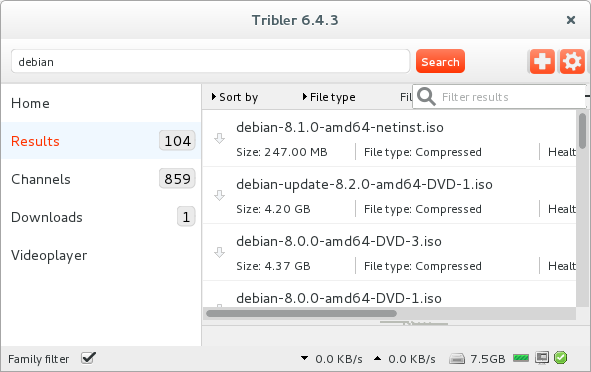
\includegraphics[scale=0.6]{introduction/figs/tribler-screenshot.png}}
%	\caption{Screenshot of Tribler v6.4.3.}
%	\label{fig:tribler-screenshot}
%\end{figure}

For years Tribler has received many contributions from students, staff and the open-source community.
This led to the degradation of structure and code quality of the Tribler code base.
Moreover, there has been done little profiling to detect bottlenecks in the code.
Finding and resolving bottlenecks in a complex code base such as Tribler's are often non-trivial yet an excellent way to increase responsiveness and performance.
For example, performing a blocking network request to a non or poorly responsive server can make the whole program grind to a halt, rendering the GUI non-responsive and leaving the user guessing what happened.
By making such a request non-blocking, the GUI remains responsive while the request is handled in the background.
In the meantime, changing such a request to become non-blocking goes well with refactoring the current structure and quality of the code to become a coherent, well-tested whole.\\

Another motivating example can be found in a recent addition to Tribler's code base.
Within Tribler anonymous connections have been recently implemented using onion routing~\cite{Plak-anonymous,ruigrok-anonymous,tanaskoski-anonymous}.
These anonymous connections are called anon-tunnels in Tribler.
This feature allows users to anonymously download files from other users in the network, safeguarding their privacy.
Every data packet has to be encrypted with multiple encryption layers and forwarded by a number of intermediate hops between the leecher and seeder~\cite{Plak-anonymous,tanaskoski-anonymous}, each decrypting one layer of encryption.
The total cost of bandwidth per file is increased, because it has to be forwarded by multiple nodes.
Because a node in the network may become part of an anon-tunnel, the workload increases per node.
The anon-tunnels have been profiled by [stokkink et al.] \todo{cite to stok et al.} and the results showed that the tunnels are now bound by CPU.
As handling packets involves encryption or decryption and message serialization, which are CPU intensive tasks, one wants to optimize this process.
The result should be higher achievable download rates and a more responsive program.

\section{Outline}
In this chapter we provided an introduction of this thesis and presented the research questions this thesis aims to answer. 
This section describes the other chapters in this thesis and their relevance to the research questions provided in section \ref{chp2:sct:objectives-research-questions}.
Chapter \ref{chp:preliminaries} provides preliminaries and terminology used through this thesis.
Chapter \ref{chp:problem-description} presents an overview of some of the problems Tribler is currently facing which this thesis addresses.
Chapter 
\todo{Add more here as cahpters are added.}
